\section{Pressure enrichment}

\subsection{Discontinuous pessure}
\begin{frame}
  \frametitle{Example ... }
  \begin{block}{}
  \end{block}
\end{frame}

\subsection{Ghost penalty}
\begin{frame}
  \frametitle{Ghost penalty}
  \begin{block}{}
  \end{block}
\end{frame}

\begin{frame}
  \frametitle{Result with ghost penalty}
  \centering
  \begin{figure}
    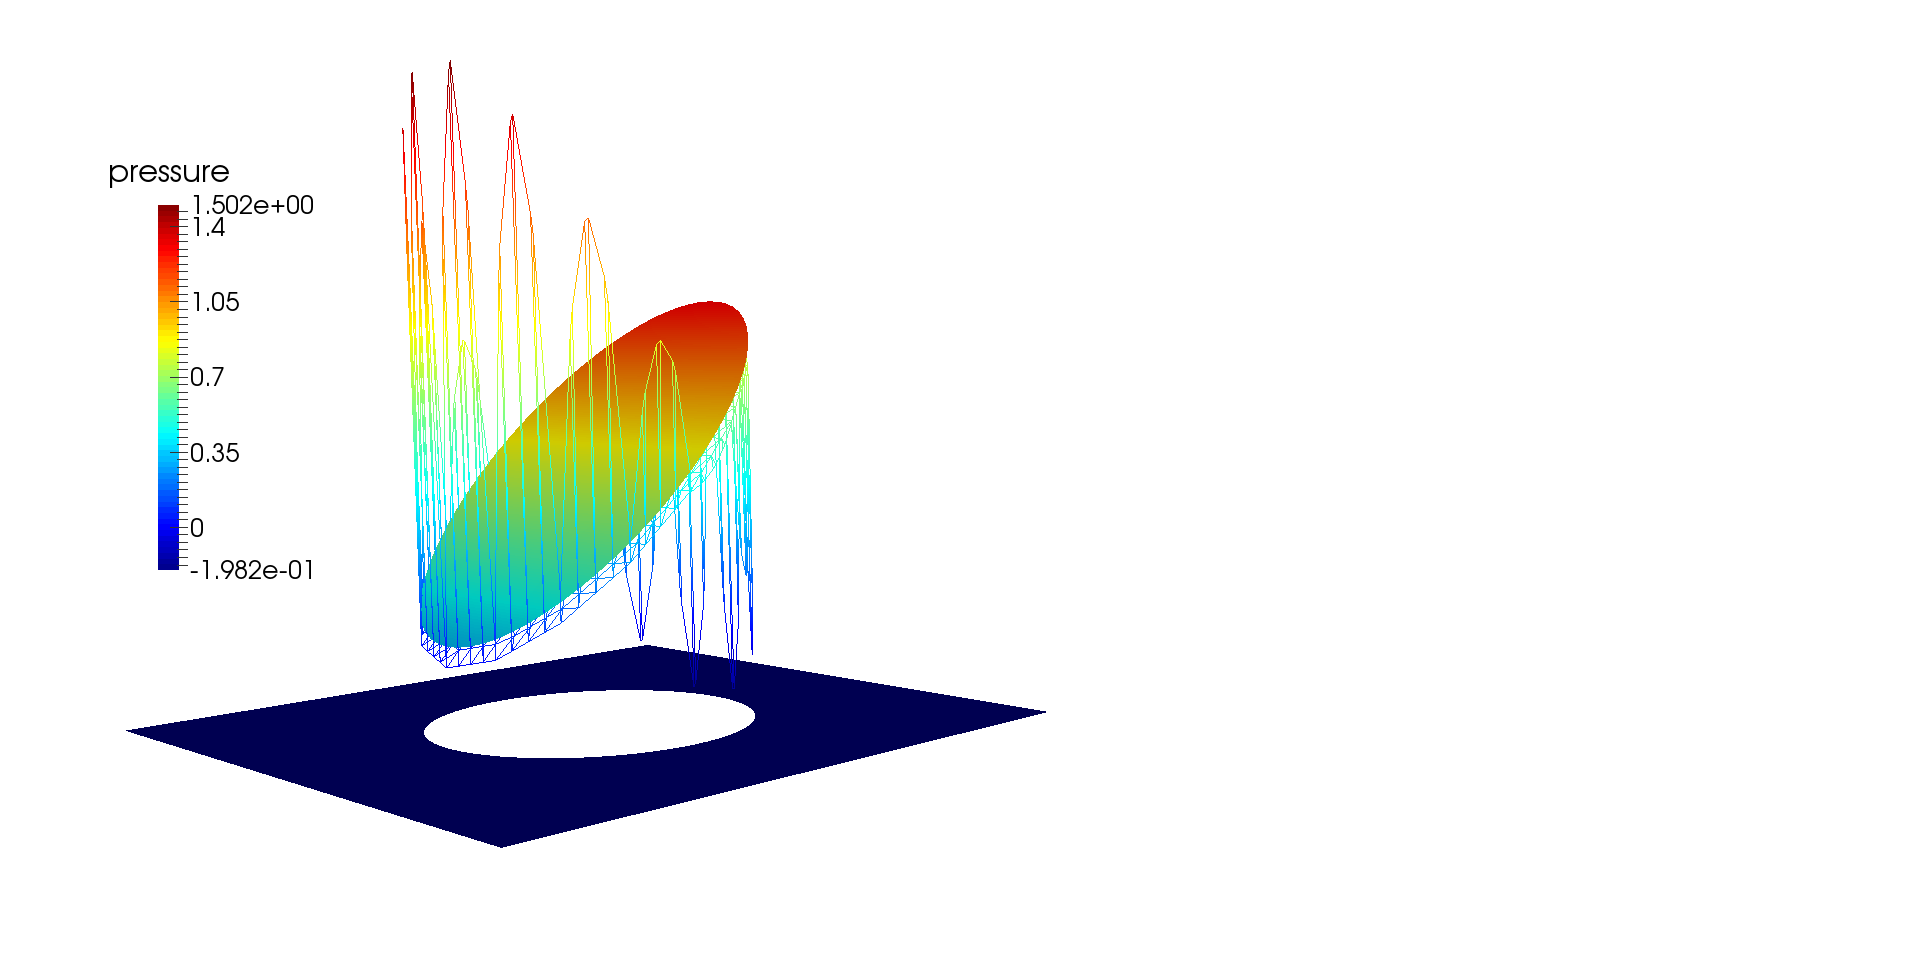
\includegraphics[height=0.5\paperheight, trim = 3cm 3cm 30cm 2cm , clip=true]{plots/together.png}
  \end{figure}
\end{frame}

%\begin{frame}
%\frametitle{Numerische Ergebnisse}
%\centering
%\vspace{-0.7cm}
%	\begin{figure}%
%		\hspace*{-0.4cm}
%		\subfloat{\includegraphics[width=0.3\paperwidth, trim = 1cm 6cm 2cm 6.5cm , clip=true]{zhab_HBrO2}}% [Bromige S�ure $\mathrm{HBrO_2}$]
%		\subfloat{\includegraphics[width=0.3\paperwidth, trim = 1cm 6cm 2cm 6.5cm , clip=true]{zhab_Br}}% [Brom $\mathrm{Br^-}$]
%		\subfloat{\includegraphics[width=0.3\paperwidth, trim = 1cm 6cm 2cm 6.5cm , clip=true]{zhab_H2O}}% [Wasser $\mathrm{H_2O}$]
%	\end{figure}%
%	\vspace{-1cm}
%	\begin{figure}%
%		\hspace*{-0.4cm}
%		\subfloat{\includegraphics[width=0.3\paperwidth, trim = 1cm 6cm 2cm 6.5cm , clip=true]{zhab_BrO3}}% [Bromat $\mathrm{BrO_3^-}$]
%		\subfloat{\includegraphics[width=0.3\paperwidth, trim = 1cm 6cm 2cm 6.5cm , clip=true]{zhab_HOBr}}% [Hypobromige S�ure $\mathrm{HBrO_2}$]
%		\visible<2->{\subfloat{\includegraphics[width=0.3\paperwidth, trim = 1cm 6cm 2cm 6.5cm , clip=true]{zhab_tau}}}% [Zeitschritt $\tau$]
%	\end{figure}
%\end{frame}
%
%\begin{frame}
%\frametitle{Grenzzyklus}
%Konzentrationen von bromiger S�ure $\mathrm{HBrO_2 = X}$, Brom $\mathrm{Br^-= Y}$ und Wasser $\mathrm{H_2O = Z}$ durchlaufen einen Grenzzyklus.
%\centering
%	\begin{figure}
%		\includegraphics[height=0.75\paperheight, trim = 0cm 0cm 0cm 2cm , clip=true]{orbit.ps}
%	\end{figure}
%\end{frame}
